\section{Sistem Kriptografi Merkle-Hellman}
\label{sec:merkle-hellman}

Karena \textit{superincreasing knapsack} terlalu mudah dipecahkan, Merkle dan
Hellman mengusulkan untuk menyembunyikannya di balik sebuah transformasi modulo.
Gagasannya bukan membuat persoalan yang baru, melainkan mengalihkan persoalan
yang sudah ada ke bentuk yang tidak lagi menampakkan sifat mudahnya. Barisan
superincreasing tetap dipakai --- tetapi hanya oleh pemilik kunci, dan hanya
dalam bentuk aslinya.

\subsection{Properti dan Kerahasiaan Parameter}

Seluruh besaran yang terlibat dirangkum pada Tabel~\ref{tab:parameter-knapsack}.

\begin{table}[htbp]
    \centering
    \begin{tabularx}{\linewidth}{@{}l
                                   >{\raggedright\arraybackslash}X
                                   c@{}}
    \toprule
    \textbf{Besaran} & \textbf{Arti} & \textbf{Rahasia?} \\
    \midrule
    $W_{priv}$ & barisan superincreasing $\{w_1, \dots, w_n\}$ & \textbf{ya} \\
    $m$ & modulus, dengan $m > \sum_i w_i$ & \textbf{ya} \\
    $n$ & pengali, dengan $\text{PBB}(n, m) = 1$ & \textbf{ya} \\
    $n^{-1}$ & invers $n$ modulo $m$ & \textbf{ya} \\
    $W_{pub}$ & barisan public $\{w'_1, \dots, w'_n\}$ & tidak \\
    $B$ & blok plainteks, $b_i \in \{0, 1\}$ & \textbf{ya} \\
    $C$ & kriptogram, $C = \sum_i b_i w'_i$ & tidak \\
    \bottomrule
    \end{tabularx}
    \caption{Besaran pada sistem Merkle--Hellman dan status kerahasiaannya.
    Perhatikan bahwa $n$ di sini adalah sebuah \emph{pengali}, bukan jumlah
    elemen; panjang barisan dituliskan secara tersirat melalui indeks $i$}
    \label{tab:parameter-knapsack}
\end{table}

Ada satu hal yang perlu diperhatikan pada Tabel~\ref{tab:parameter-knapsack}.
Yang dirahasiakan bukan hanya barisan bobotnya, melainkan juga $m$ dan $n$.
Kedua parameter itu adalah pintu jebakan itu sendiri: tanpa keduanya, barisan
publik tidak dapat dikembalikan ke wujud superincreasing-nya. Sebaliknya,
barisan publik memang dirancang untuk disiarkan, sebab dari situlah pengirim
membaca mana elemen yang harus dijumlahkan.

\subsection{Pembangkitan Kunci}

Langkah-langkah pembangkitan kunci adalah sebagai berikut.

\begin{enumerate}
    \item \textbf{Kunci Privat}: Pilih sebuah barisan \textit{superincreasing} $W_{priv} = \{w_1, w_2, \dots, w_n\}$.
    \item \textbf{Parameter Transformasi}: Pilih modulus $m$ yang lebih besar dari jumlah seluruh elemen $W_{priv}$, dan pilih pengali $n$ sedemikian sehingga $\text{PBB}(n, m) = 1$.
    \item \textbf{Kunci Publik}: Hitung barisan \textit{non-superincreasing} $W_{pub} = \{w'_1, w'_2, \dots, w'_n\}$ dengan rumus:
    \begin{equation}
    w'_i = (w_i \cdot n) \bmod m .
    \label{eq:mh-kunci}
    \end{equation}
\end{enumerate}

Kedua syarat pada langkah 2 bukan syarat administratif, melainkan penopang
seluruh mekanisme. Syarat $m > \sum_i w_i$ menjamin bahwa penjumlahan seluruh
elemen barisan privat tidak pernah ``memutar'' melewati modulus; tanpa syarat
itu, hasil dekripsi dapat berbeda dari nilai sebenarnya modulo $m$, dan
algoritma \textit{greedy} akan menerima sisa yang keliru
(Subbagian~\ref{subsec:bukti-knapsack}). Syarat $\text{PBB}(n, m) = 1$
menjamin bahwa $n$ memiliki invers modulo $m$. Bila kedua bilangan itu punya
faktor persekutuan, inversnya tidak ada, dan penerima yang sah sama sekali
tidak dapat mendekripsi pesan --- kerusakan yang baru ketahuan setelah seluruh
pesan terkirim.

Perhatikan pula bahwa hasil Persamaan~\eqref{eq:mh-kunci} memang tidak lagi
superincreasing. Pengambilan modulo $m$ mengacak urutan besar-kecilnya, sebab
sebuah elemen yang tadinya kecil dapat terpental hampir ke $m - 1$ bila
$w_i \cdot n$ kebetulan sedikit di bawah kelipatan $m$. Justru pengacakan
itulah yang diharapkan: di mata penyadap, $W_{pub}$ tampak seperti barisan
bilangan acak biasa, dan menaksir $M = \sum_i b_i w'_i$ dari barisan semacam itu
kembali menjadi persoalan yang sulit.

\subsection{Proses Enkripsi}

Pengirim menggunakan kunci publik $W_{pub}$ untuk mengenkripsi pesan biner
$B = (b_1, b_2, \dots, b_n)$:

\begin{equation}
C = \sum_{i=1}^{n} b_i w'_i .
\label{eq:mh-enkripsi}
\end{equation}

Hasil enkripsi adalah sebuah angka tunggal $C$ (kriptogram). Cara kerjanya
sama dengan knapsack sederhana pada Bagian~\ref{sec:masalah-knapsack}: bit yang
bernilai $1$ menyumbangkan elemen publiknya, bit yang bernilai $0$ tidak.

Satu catatan perlu diberikan mengenai modulus pada
Persamaan~\eqref{eq:mh-enkripsi}. Berbeda dari enkripsi ElGamal pada bab
sebelumnya, penjumlahan di sini \textbf{tidak} diambil modulo $m$. Nilai $C$
dibiarkan apa adanya, sehingga ia sering lebih besar daripada $m$ --- dan itu
memang tidak menjadi masalah. Alasannya, dekripsi nanti hanya memakai
$C \bmod m$, sehingga pengurangan modulo $m$ di sisi pengirim tidak mengubah
hasil apa pun; keduanya sama-sama sah. Yang perlu dipastikan hanyalah agar
pengirim dan penerima memakai kesepakatan yang sama, sebab bila salah satu
mengurangi dan yang lain tidak, nilai $C$ yang diuji akan berbeda walaupun
residunya sama.

Karena setiap blok menghasilkan satu bilangan, panjang pesan menentukan banyak
blok, dan setiap blok harus sepanjang $n$ bit --- yaitu sebanyak elemen di dalam
kunci publik. Pesan yang panjangnya bukan kelipatan $n$ perlu diberi
\textit{padding}, persis seperti pada RSA dan ElGamal.

\subsection{Proses Dekripsi}

Penerima menggunakan kunci privat $W_{priv}$ dan parameter $(n, m)$ untuk
mendekripsi:

\begin{enumerate}
    \item Hitung invers modulo dari $n$ terhadap $m$, yaitu $n^{-1} \bmod m$.
    \item Transformasikan kriptogram $C$ kembali menjadi bentuk \textit{superincreasing}:
    \begin{equation}
    C' = (C \cdot n^{-1}) \bmod m .
    \label{eq:mh-dekripsi}
    \end{equation}
    \item Pecahkan $C'$ menggunakan algoritma \textit{greedy} terhadap barisan $W_{priv}$ untuk mendapatkan bit-bit plainteks $b_i$.
\end{enumerate}

\subsection{Mengapa Dekripsi Berhasil}
\label{subsec:bukti-knapsack}

Langkah 2 pada prosedur di atas adalah inti seluruh sistem, dan kebenarannya
perlu diperlihatkan. Substitusikan Persamaan~\eqref{eq:mh-enkripsi} ke dalam
Persamaan~\eqref{eq:mh-dekripsi}:

\begin{equation}
\begin{split}
C' &\equiv n^{-1} \sum_{i=1}^{n} b_i w'_i \pmod{m} \\
   &\equiv n^{-1} \sum_{i=1}^{n} b_i (w_i n) \pmod{m} \\
   &\equiv \sum_{i=1}^{n} b_i w_i \pmod{m} .
\end{split}
\label{eq:mh-bukti}
\end{equation}

Pada baris kedua, rumus pembangkitan kunci dari
Persamaan~\eqref{eq:mh-kunci} telah dipakai; pada baris ketiga, faktor $n^{-1}$
dan $n$ saling meniadakan sehingga yang tersisa hanyalah jumlah berbobot elemen
privat --- tepat seperti Persamaan~\eqref{eq:knapsack-dasar}.

Sampai di sini yang diperoleh baru kesamaan \emph{modulo} $m$. Agar algoritma
\textit{greedy} dapat dipakai, kesamaan itu harus ditingkatkan menjadi kesamaan
yang sesungguhnya. Di sinilah syarat $m > \sum_i w_i$ bekerja. Karena setiap
$b_i$ bernilai $0$ atau $1$,

\[ 0 \le \sum_{i=1}^{n} b_i w_i \le \sum_{i=1}^{n} w_i < m , \]

sehingga jumlah itu sudah berada di dalam selang $[0, m-1]$ dan tidak mungkin
memutar melewati modulus. Akibatnya tidak ada dua nilai berbeda yang memberi
residu yang sama, dan Persamaan~\eqref{eq:mh-bukti} dapat ditulis sebagai
kesamaan biasa:

\begin{equation}
C' = \sum_{i=1}^{n} b_i w_i .
\label{eq:mh-bukti-eksak}
\end{equation}

Dengan kata lain, mengalikan kriptogram dengan $n^{-1}$ modulo $m$ mengubah
kembali persoalan yang tampak sulit menjadi persoalan superincreasing yang
sudah dikenal. Seluruh kekuatan sistem Merkle--Hellman terletak pada satu
kenyataan itu: penerima tidak pernah perlu memecahkan knapsack publik, sebab
ia memegang $n^{-1}$ yang membuat knapsack itu lenyap.

Kebalikannya juga berlaku, dan di situlah letak kerawanannya. Seorang penyerang
yang berhasil menebak pasangan $(n, m)$ yang benar dapat melakukan tepat
langkah yang sama seperti penerima, dan seluruh pesan terbuka untuknya. Jadi
keamanan sistem ini sesungguhnya bergantung pada sulitnya menemukan $n^{-1}$
tanpa mengetahui $n$, bukan pada sulitnya persoalan knapsack secara umum.
Bagian~\ref{sec:kriptanalisis-knapsack} memperlihatkan bahwa Shamir berhasil
menemukannya.

% Alur sistem kriptografi Merkle-Hellman (knapsack).
% Dirujuk dari section-03.tex dengan % Alur sistem kriptografi Merkle-Hellman (knapsack).
% Dirujuk dari section-03.tex dengan % Alur sistem kriptografi Merkle-Hellman (knapsack).
% Dirujuk dari section-03.tex dengan \input{figures/alur-knapsack}.
\begin{figure}[htbp]
    \centering
    % Diagram ini lebih lebar dari \linewidth, jadi diskalakan agar tidak
    % menimbulkan Overfull \hbox (lebar teks: 21cm - 3cm - 2,5cm = 15,5cm).
    \resizebox{0.97\linewidth}{!}{%
    \begin{tikzpicture}[
        kotak/.style={draw, rounded corners, align=center, font=\small, inner sep=5pt},
        panah/.style={-{Latex[length=2.4mm]}, thick},
        kunci/.style={-{Latex[length=2.4mm]}, thick, dashed, gray!75},
    ]
        % Baris 1: transformasi kunci privat menjadi kunci publik
        \node[kotak, fill=red!6, minimum width=4.2cm] (priv) at (0,0)
            {Kunci privat: barisan\\ \textit{superincreasing} $W_{priv}$};
        \node[kotak, fill=orange!12, minimum width=3.4cm] (tr) at (5.4,0)
            {$w'_i = (w_i \cdot n) \bmod m$};
        \node[kotak, fill=blue!6, minimum width=4.2cm] (pub) at (10.6,0)
            {Kunci publik: barisan\\ $W_{pub}$ (non-\textit{superincreasing})};

        \draw[panah] (priv) -- node[above, font=\scriptsize] {$n, m$} (tr);
        \draw[panah] (tr) -- (pub);

        % Baris 2: enkripsi dan dekripsi
        \node[kotak, fill=green!10, minimum width=3.0cm] (msg) at (-2.9,-2.6)
            {Pesan biner\\ $B = (b_1, \dots, b_n)$};
        \node[kotak, fill=orange!12, minimum width=3.6cm] (enc) at (0.9,-2.6)
            {$C = \sum_i b_i w'_i \bmod m$};
        \node[kotak, fill=green!10, minimum width=1.6cm] (c) at (3.8,-2.6) {$C$};
        \node[kotak, fill=orange!12, minimum width=4.4cm] (dec) at (7.4,-2.6)
            {$C' = C \cdot n^{-1} \bmod m$,\\ lalu dipecahkan secara \textit{greedy}};
        \node[kotak, fill=green!10, minimum width=3.0cm] (msg2) at (11.6,-2.6)
            {Pesan biner\\ $B = (b_1, \dots, b_n)$};

        \draw[kunci] (pub.south)  -- ++(0,-0.35) -| (enc.north);
        \draw[kunci] (priv.south) -- ++(0,-0.35) -| (dec.north);

        \draw[panah] (msg) -- (enc);
        \draw[panah] (enc) -- (c);
        \draw[panah] (c) -- (dec);
        \draw[panah] (dec) -- (msg2);
    \end{tikzpicture}%
    }
    \caption{Alur sistem Merkle-Hellman: kunci privat \textit{superincreasing} disamarkan menjadi kunci publik, enkripsi memakai kunci publik, sedangkan dekripsi menuntut kunci privat}
    \label{fig:alur-knapsack}
\end{figure}
.
\begin{figure}[htbp]
    \centering
    % Diagram ini lebih lebar dari \linewidth, jadi diskalakan agar tidak
    % menimbulkan Overfull \hbox (lebar teks: 21cm - 3cm - 2,5cm = 15,5cm).
    \resizebox{0.97\linewidth}{!}{%
    \begin{tikzpicture}[
        kotak/.style={draw, rounded corners, align=center, font=\small, inner sep=5pt},
        panah/.style={-{Latex[length=2.4mm]}, thick},
        kunci/.style={-{Latex[length=2.4mm]}, thick, dashed, gray!75},
    ]
        % Baris 1: transformasi kunci privat menjadi kunci publik
        \node[kotak, fill=red!6, minimum width=4.2cm] (priv) at (0,0)
            {Kunci privat: barisan\\ \textit{superincreasing} $W_{priv}$};
        \node[kotak, fill=orange!12, minimum width=3.4cm] (tr) at (5.4,0)
            {$w'_i = (w_i \cdot n) \bmod m$};
        \node[kotak, fill=blue!6, minimum width=4.2cm] (pub) at (10.6,0)
            {Kunci publik: barisan\\ $W_{pub}$ (non-\textit{superincreasing})};

        \draw[panah] (priv) -- node[above, font=\scriptsize] {$n, m$} (tr);
        \draw[panah] (tr) -- (pub);

        % Baris 2: enkripsi dan dekripsi
        \node[kotak, fill=green!10, minimum width=3.0cm] (msg) at (-2.9,-2.6)
            {Pesan biner\\ $B = (b_1, \dots, b_n)$};
        \node[kotak, fill=orange!12, minimum width=3.6cm] (enc) at (0.9,-2.6)
            {$C = \sum_i b_i w'_i \bmod m$};
        \node[kotak, fill=green!10, minimum width=1.6cm] (c) at (3.8,-2.6) {$C$};
        \node[kotak, fill=orange!12, minimum width=4.4cm] (dec) at (7.4,-2.6)
            {$C' = C \cdot n^{-1} \bmod m$,\\ lalu dipecahkan secara \textit{greedy}};
        \node[kotak, fill=green!10, minimum width=3.0cm] (msg2) at (11.6,-2.6)
            {Pesan biner\\ $B = (b_1, \dots, b_n)$};

        \draw[kunci] (pub.south)  -- ++(0,-0.35) -| (enc.north);
        \draw[kunci] (priv.south) -- ++(0,-0.35) -| (dec.north);

        \draw[panah] (msg) -- (enc);
        \draw[panah] (enc) -- (c);
        \draw[panah] (c) -- (dec);
        \draw[panah] (dec) -- (msg2);
    \end{tikzpicture}%
    }
    \caption{Alur sistem Merkle-Hellman: kunci privat \textit{superincreasing} disamarkan menjadi kunci publik, enkripsi memakai kunci publik, sedangkan dekripsi menuntut kunci privat}
    \label{fig:alur-knapsack}
\end{figure}
.
\begin{figure}[htbp]
    \centering
    % Diagram ini lebih lebar dari \linewidth, jadi diskalakan agar tidak
    % menimbulkan Overfull \hbox (lebar teks: 21cm - 3cm - 2,5cm = 15,5cm).
    \resizebox{0.97\linewidth}{!}{%
    \begin{tikzpicture}[
        kotak/.style={draw, rounded corners, align=center, font=\small, inner sep=5pt},
        panah/.style={-{Latex[length=2.4mm]}, thick},
        kunci/.style={-{Latex[length=2.4mm]}, thick, dashed, gray!75},
    ]
        % Baris 1: transformasi kunci privat menjadi kunci publik
        \node[kotak, fill=red!6, minimum width=4.2cm] (priv) at (0,0)
            {Kunci privat: barisan\\ \textit{superincreasing} $W_{priv}$};
        \node[kotak, fill=orange!12, minimum width=3.4cm] (tr) at (5.4,0)
            {$w'_i = (w_i \cdot n) \bmod m$};
        \node[kotak, fill=blue!6, minimum width=4.2cm] (pub) at (10.6,0)
            {Kunci publik: barisan\\ $W_{pub}$ (non-\textit{superincreasing})};

        \draw[panah] (priv) -- node[above, font=\scriptsize] {$n, m$} (tr);
        \draw[panah] (tr) -- (pub);

        % Baris 2: enkripsi dan dekripsi
        \node[kotak, fill=green!10, minimum width=3.0cm] (msg) at (-2.9,-2.6)
            {Pesan biner\\ $B = (b_1, \dots, b_n)$};
        \node[kotak, fill=orange!12, minimum width=3.6cm] (enc) at (0.9,-2.6)
            {$C = \sum_i b_i w'_i \bmod m$};
        \node[kotak, fill=green!10, minimum width=1.6cm] (c) at (3.8,-2.6) {$C$};
        \node[kotak, fill=orange!12, minimum width=4.4cm] (dec) at (7.4,-2.6)
            {$C' = C \cdot n^{-1} \bmod m$,\\ lalu dipecahkan secara \textit{greedy}};
        \node[kotak, fill=green!10, minimum width=3.0cm] (msg2) at (11.6,-2.6)
            {Pesan biner\\ $B = (b_1, \dots, b_n)$};

        \draw[kunci] (pub.south)  -- ++(0,-0.35) -| (enc.north);
        \draw[kunci] (priv.south) -- ++(0,-0.35) -| (dec.north);

        \draw[panah] (msg) -- (enc);
        \draw[panah] (enc) -- (c);
        \draw[panah] (c) -- (dec);
        \draw[panah] (dec) -- (msg2);
    \end{tikzpicture}%
    }
    \caption{Alur sistem Merkle-Hellman: kunci privat \textit{superincreasing} disamarkan menjadi kunci publik, enkripsi memakai kunci publik, sedangkan dekripsi menuntut kunci privat}
    \label{fig:alur-knapsack}
\end{figure}


\begin{figure}[htbp]
    \centering
    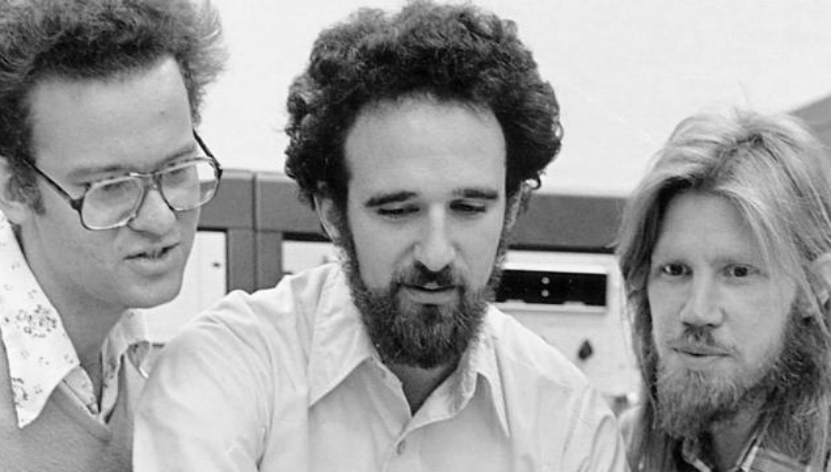
\includegraphics[width=0.7\linewidth, height=0.45\textheight, keepaspectratio]{figures/perumus-knapsack.png}
    \caption{Ralph Merkle, Martin Hellman, dan Whitfield Diffie, para perumus sistem knapsack Merkle-Hellman dan protokol pertukaran kunci Diffie-Hellman}
    \label{fig:perumus-knapsack}
    \sumber{Munir, \textit{IF4020 Kriptografi}, ITB.}
\end{figure}
